\documentclass[aspectratio=169]{beamer}
\usepackage{will_handley_beamer}
\usepackage{title_page}
\usetikzlibrary{positioning}
\usetikzlibrary{calc}
\usetikzlibrary{fit}

% Commands
% --------
% - \arxiv{arxiv number}
% - \cols{width}{lh column}{rh column}
% -  \begin{fig(left|right)}[fractional width (e.g 0.6) ]{name of image}
%        content of other column
%    \end{fig(left|right)}

% Talk details
% ------------
\title{Simulation Based Inference}
\subtitle{sampling, model comparison, \& amortisation}
\date{12\textsuperscript{th} January 2024}

\begin{document}

\begin{frame}
    \titlepage
\end{frame}

\begin{frame}
    \frametitle{How all SBI talks finish}
    \begin{itemize}
        \item There is a standard exchange that tends to happen after giving an SBI talk:

            \begin{description}
                \item[audience] Surely you're only as good as your simulations ---\\What if your forward model is missing physics $X$?
                \item[speaker] The exact same thing affects likelihood-based analysis ---\\
                    All SBI does is make these assumptions explicit.
            \end{description}
        \item I will try to unpack why I think both sides have a point.
    \end{itemize}
    \vspace{10pt}
\hfill \textit{Frontiers of simulation based inference}~\arxiv{1911.01429}
    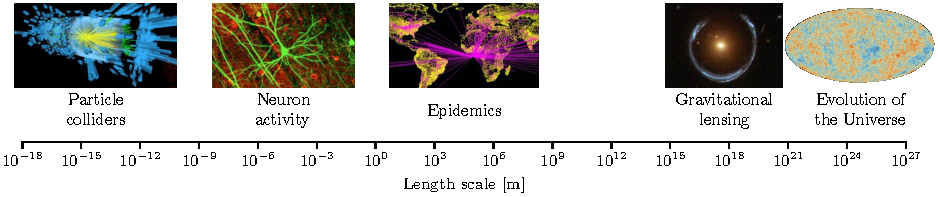
\includegraphics[width=\textwidth]{figures/sbi_range.pdf}
\end{frame}

\begin{frame}
    \frametitle{LBI: Likelihood-based inference}
    \begin{columns}
        \column{0.5\textwidth}
The standard approach if you are fortunate enough to have a likelihood function $\only<1-2>{P}\only<3->{\mathcal{L}}(\theta|D)$: 
        \[
            \only<1-2>{
                P(\theta|D) = \frac{P(D|\theta)P(\theta)}{P(D)}
        }
            \only<2>{
            \qquad
            \text{Posterior} = \frac{\text{Likelihood}\times\text{Prior}}{\text{Evidence}}
        }
            \only<3>{
                \mathcal{P}(\theta|D) = \frac{\mathcal{L}(D|\theta)\pi(\theta)}{\mathcal{Z}(D)}
            \qquad
            \text{Posterior} = \frac{\text{Likelihood}\times\text{Prior}}{\text{Evidence}}
        }
            \only<4>{
                \mathcal{P}\times\mathcal{Z} = \mathcal{L}\times\pi
        }
            \only<5>{
                \mathcal{P}\times\mathcal{Z} = \mathcal{J} = \mathcal{L}\times\pi, \qquad \text{Joint} = \mathcal{J} = P(D,\theta)
        }
        \]
        \vspace{-10pt}
        \begin{enumerate}
            \item Define prior $\pi(\theta)$ 
                \begin{itemize}
                    \item spend some time being philosophical
                \end{itemize}
            \item Sample posterior $\mathcal{P}(\theta|D)$ 
                \begin{itemize}
                    \item use out-of-the-box MCMC tools such as\\ \texttt{emcee} or \texttt{MultiNest}
                    \item make some triangle plots
                \end{itemize}
            \item Optionally compute evidence $\mathcal{Z}(D)$
                \begin{itemize}
                    \item e.g. nested sampling or parallel tempering
                    \item do some model comparison (i.e. science)
                    \item talk about tensions e.g. \arxiv{2401.02929}
                \end{itemize}
        \end{enumerate}
        \column{0.5\textwidth}
        \hfill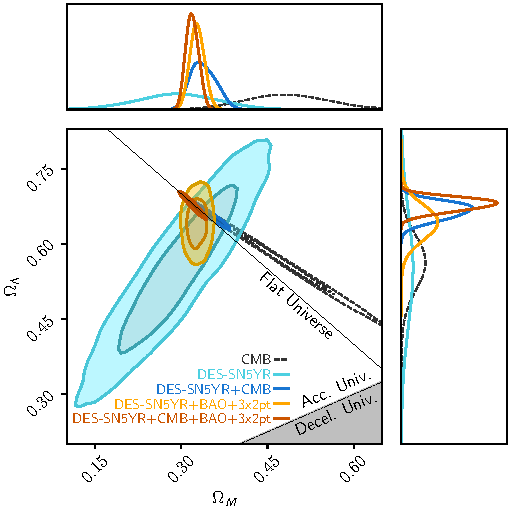
\includegraphics[width=0.6\textwidth]{figures/des_parameters.pdf}
        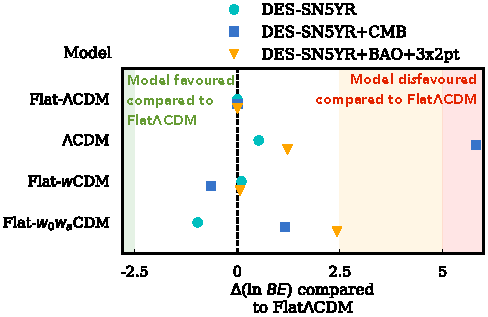
\includegraphics[width=0.5\textwidth]{figures/des_model_comparison.pdf}%
        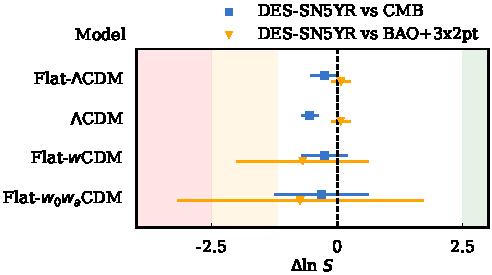
\includegraphics[width=0.5\textwidth]{figures/des_suspiciousness.pdf}
    \end{columns}
\end{frame}

\begin{frame}
    \frametitle{SBI: Simulation-based inference}
    \begin{columns}
        \column{0.5\textwidth}
        \begin{itemize}
            \item Only have access to a forward model $\theta \rightarrow D$.
            \item $(\theta,D)$ plane gives a more expansive theoretical view of inference.
            \item Forward model defines \emph{implicit} likelihood~$\mathcal{L}$:
            \item Simulator generates samples from $\mathcal{L}(D|\theta)$.
            \item With a prior $\pi(\theta)$ can generate samples from joint distribution~$\mathcal{J}(\theta,D)=\mathcal{L}(D|\theta)\pi(\theta)$\\\hfill \emph{the ``probability of everything''}.
            \item Task of SBI is then to go from joint~$\mathcal{J}$ to posterior $\mathcal{P}(\theta|D)$ and evidence $\mathcal{Z}(D)$ -- and possibly likelihood $\mathcal{L}(D|\theta)$.
            \item SBI \& forward modelling force us to think about data space~$D$ \& parameter space~$\theta$.
        \end{itemize}
        \column{0.5\textwidth}
        \includegraphics<1>[page=1, width=\textwidth]{figures/sbi_parameter_estimation.pdf}%
        \includegraphics<2>[page=2, width=\textwidth]{figures/sbi_parameter_estimation.pdf}%
        \includegraphics<3>[page=3, width=\textwidth]{figures/sbi_parameter_estimation.pdf}%
        \includegraphics<4>[page=4, width=\textwidth]{figures/sbi_parameter_estimation.pdf}%
        \includegraphics<5>[page=5, width=\textwidth]{figures/sbi_parameter_estimation.pdf}%
    \end{columns}
\end{frame}


\begin{frame}
    \frametitle{Simulation-based inference \& model comparison}
    \begin{columns}
        \column{0.3\textwidth}
        \begin{itemize}
            \item Extend: models $A$ and $B$.
            \item Each with own separate parameters $\theta_A$ and $\theta_B$ (can be same).
            \item The evidence $\mathcal{Z}(D|M)$ compares models
            \item Occams razor: more~predictive $\equiv$~more~probable \\(due to normalisation).
        \end{itemize}
        
        \column{0.7\textwidth}
        \includegraphics<1>[page=1, width=\textwidth]{figures/sbi_model_comparison.pdf}%
        \includegraphics<2>[page=2, width=\textwidth]{figures/sbi_model_comparison.pdf}%
        \includegraphics<3>[page=3, width=\textwidth]{figures/sbi_model_comparison.pdf}%
    \end{columns}
\end{frame}

\begin{frame}
    \frametitle{Evidence networks~\arxiv{2305.11241}}
    \begin{columns}
        \column{0.5\textwidth}
    \begin{itemize}
        \item Procedure proposed by Jeffreys \& Wandelt:
            \begin{enumerate}
                \item Generate labelled data from model $A$ and model $B$.
                \item Train a probabilistic classifier to distinguish between the two.
                \item Use neural ratio trick to extract Bayes Factor $B = P(D|A)/P(D|B)$.
            \end{enumerate}
        \item NRE for data
        \item Fully marginalises out parameters
        \item Only works in the data space
        \item Model comparison without nested sampling!
        \item Can be extremely effective
    \end{itemize}
        
        \column{0.5\textwidth}
        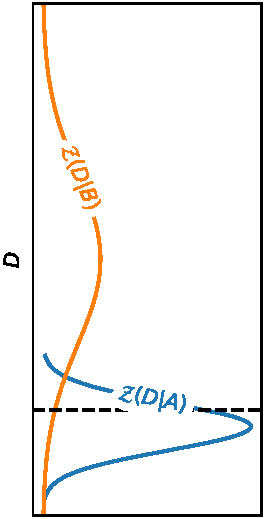
\includegraphics[width=0.5\textwidth]{figures/sbi-0.pdf}%
        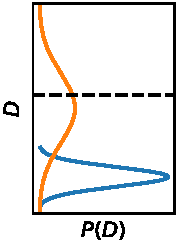
\includegraphics[width=0.5\textwidth]{figures/sbi-1.pdf}
    \end{columns}
\end{frame}

\begin{frame}
    \frametitle{A word of caution on data-space modelling}
    \begin{columns}
        \column{0.3\textwidth}
        \begin{itemize}
            \item In practice the situation is more like this $\Rightarrow$
                \begin{itemize}
                    \item \emph{``No models are true,} \\\emph{(but some are useful)''}
                \end{itemize}
            \item Curse of dimensionality means real data may not lie in either/any evidence distribution $\mathcal{Z}(D)$.
            \item e.g. if you are training an ML method, it will have never seen simulated data like the real data.
        \end{itemize}
        
        \column{0.7\textwidth}
        %\includegraphics<1>[page=4, width=\textwidth]{figures/sbi_model_comparison.pdf}%
        \includegraphics[page=5, width=\textwidth]{figures/sbi_model_comparison.pdf}%
    \end{columns}
\end{frame}

\begin{frame}
    \frametitle{A word of caution on data-space modelling}
            \begin{columns}
                \column{0.5\textwidth}
    \begin{itemize}
        \item This concern affects any amortised method 
            \begin{itemize}
                \item means trainining method on simulations\ldots
                \item \ldots and then pass in the real data
                \item They are amortised (over the data) because they can be re-used for any new data.
            \end{itemize}
        \item Observed data is only thing we surely know.
        \item As scientists we should be suspicious of a method that leaves $D_\mathrm{obs}$ until the end.
        \item This can be amelioriated by fitting $\theta$.
            \begin{itemize}
                \item Fitting concentrates parameters \& simulations around the posterior/real data
                \item See this in truncated approaches \& ABC
            \end{itemize}
    \end{itemize}
                \column{0.5\textwidth}
                \includegraphics[page=6, width=\textwidth]{figures/sbi_parameter_estimation.pdf}%
            \end{columns}

\end{frame}

\begin{frame}
    \frametitle{Why do amortised methods often work so well?}
        Whilst these concerns sound worrying, many succesful amortised methods exist. Why?
    \begin{enumerate}
        \item Some methods are only validated on data generated from the same simulator as the one used for inference.
        \item Some methods are only validated on simple Gaussian examples, since it's possible to compute the ground truth in these cases.
            \begin{itemize}
                \item Recommendation: also test on Gaussian mixture models, for which full analytics are also known
            \end{itemize}
        \item Real data may not actually be that challenging!
    \end{enumerate}
\end{frame}
\begin{frame}
    \frametitle{\texttt{lsbi}: Linear Simulation Based Inference}
    \begin{columns}
        \column{0.5\textwidth}
        \begin{itemize}
            \item If the final point holds, then in many cases we may not need expressive ML/AI methods
            \item Often it is the data-intensive ``plug-and-play'' power of ML packages that is most useful.
            \item If your ML is just learning a simple decision boundary, why not just use a linear model?
            \item \texttt{lsbi} is a python package that implements plug-and-play the fiddly linear mathematics.
            \item Also pedagogically useful for persuading people that SBI $\ne$ ML.
            \item Beta-testers wanted:
            \item \texttt{lsbi}: \href{https://github.com/handley-lab/lsbi}{github.com/handley-lab/lsbi}\\ (PyPI \& conda)
        \end{itemize}
        \column{0.5\textwidth}
        \includegraphics<1>[width=\textwidth]{figures/gaussian.png}%
        \includegraphics<2>[width=\textwidth]{figures/needles.png}%
        \includegraphics<3>[width=\textwidth]{figures/ring.png}%
    \end{columns}
\end{frame}



\begin{frame}
    \frametitle{How this SBI talk finishes}
    \begin{itemize}
        \item There is a standard exchange that tends to happen after giving an SBI talk:

            \begin{description}
                \item[audience] Surely you're only as good as your simulations ---\\What if your forward model is missing physics $X$?
                \item[speaker] The exact same thing affects likelihood-based analysis ---\\
                    All SBI does is make these assumptions explicit.
            \end{description}
        \item The audience is implicitly making a query about the danger of working in data space~$D$, whilst the speaker's comment only applies to parameter space $\theta$.
        \item Discussion point: We should therefore focus on SBI approaches which have tunable parameter spaces (i.e. interpretable posteriors).
    \end{itemize}
\end{frame}


\begin{frame}
    \frametitle{Conclusions}
    \framesubtitle{\href{https://www.github.com/handley-lab}{github.com/handley-lab}}
    \tikz[overlay,remember picture]
        \node[anchor=north east] (A) at ($(current page.north east)+(0,0)$) {
            
\includegraphics[width=0.09\textheight]{figures/students/adam_ormondroyd.jpg}%
            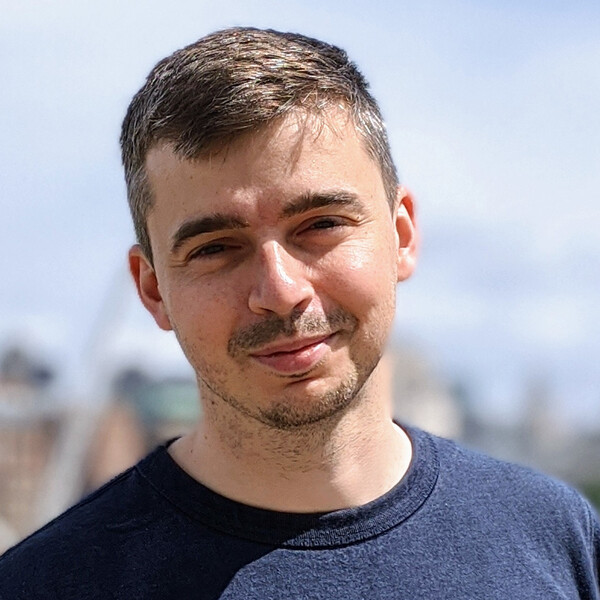
\includegraphics[width=0.09\textheight]{figures/students/david_yallup.jpg}%
            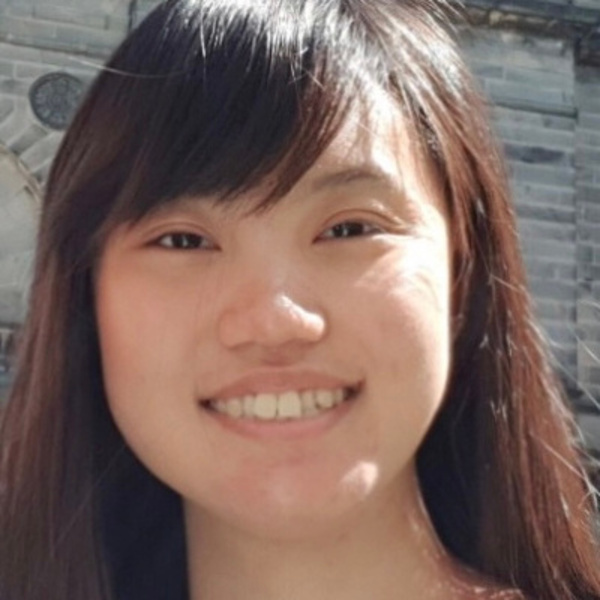
\includegraphics[width=0.09\textheight]{figures/students/dily_ong.jpg}%
            
\includegraphics[width=0.09\textheight]{figures/students/felicity_ibrahim.jpg}%
            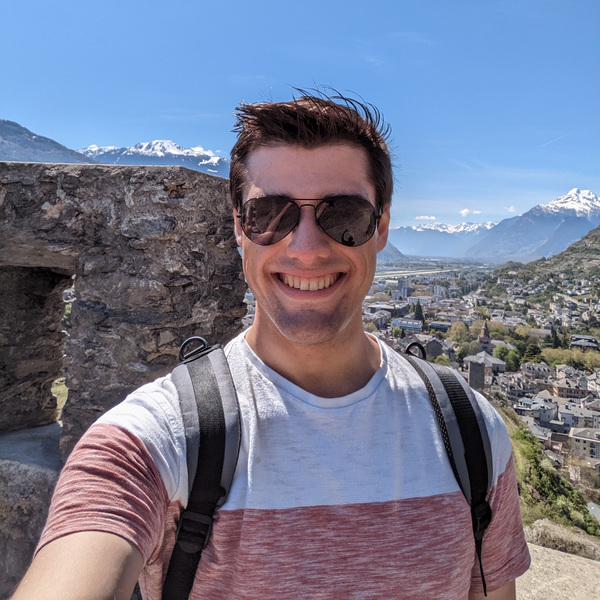
\includegraphics[width=0.09\textheight]{figures/students/george_carter.jpg}%
            
\includegraphics[width=0.09\textheight]{figures/students/harry_bevins.jpg}%
            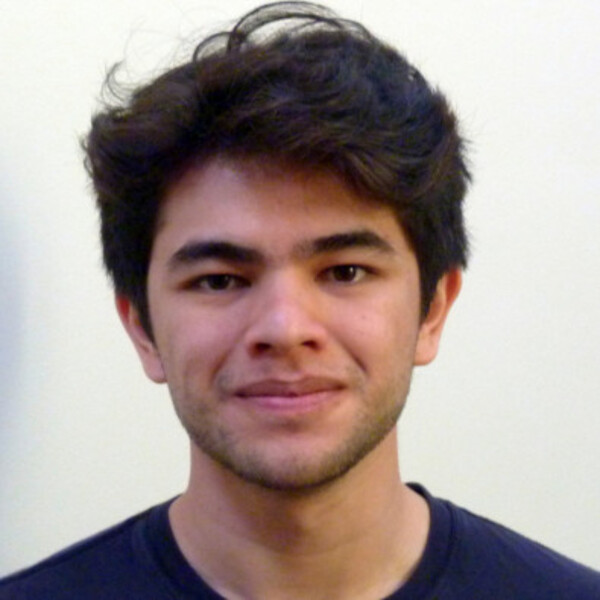
\includegraphics[width=0.09\textheight]{figures/students/ian_roque.jpg}%
            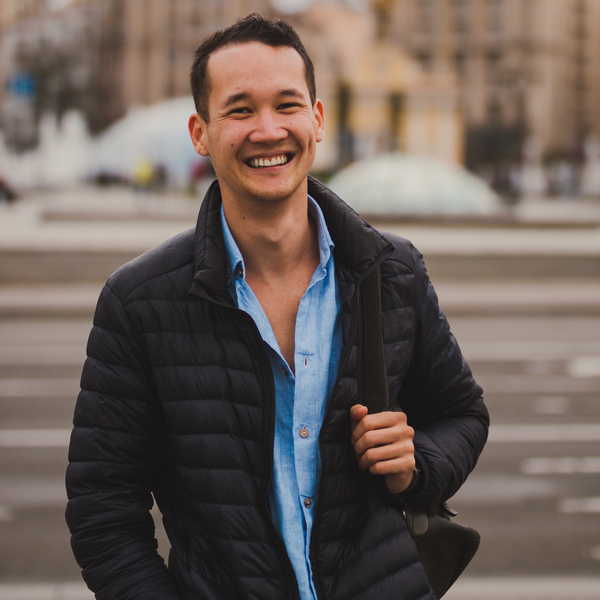
\includegraphics[width=0.09\textheight]{figures/students/kilian_scheutwinkel.jpg}%
            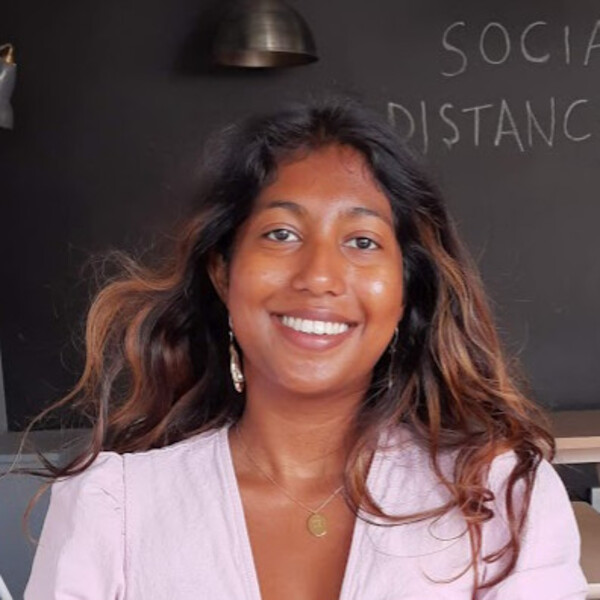
\includegraphics[width=0.09\textheight]{figures/students/metha_prathaban.jpg}%
            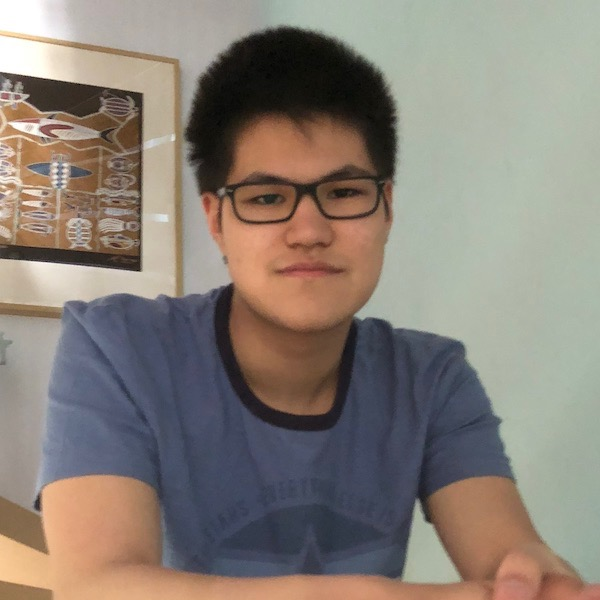
\includegraphics[width=0.09\textheight]{figures/students/namu_kroupa.jpg}%
            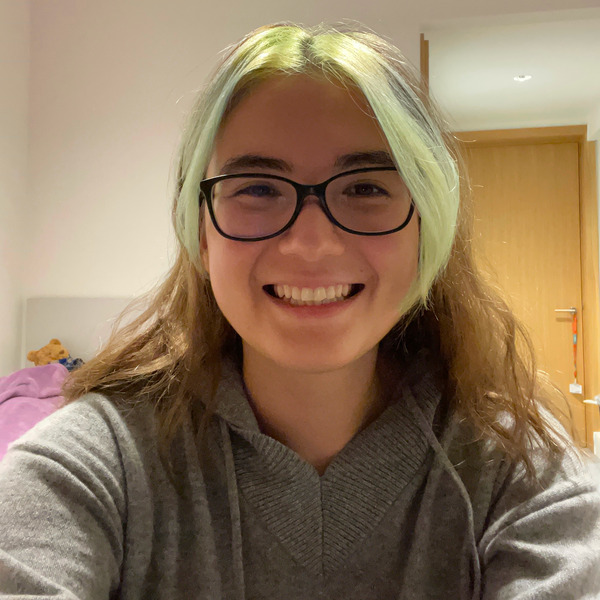
\includegraphics[width=0.09\textheight]{figures/students/sinah_legner.jpg}%
            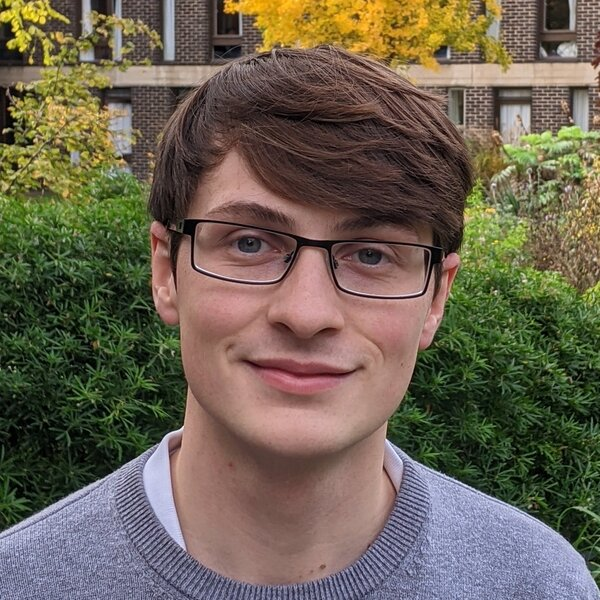
\includegraphics[width=0.09\textheight]{figures/students/thomas_gessey-jones.jpg}%
            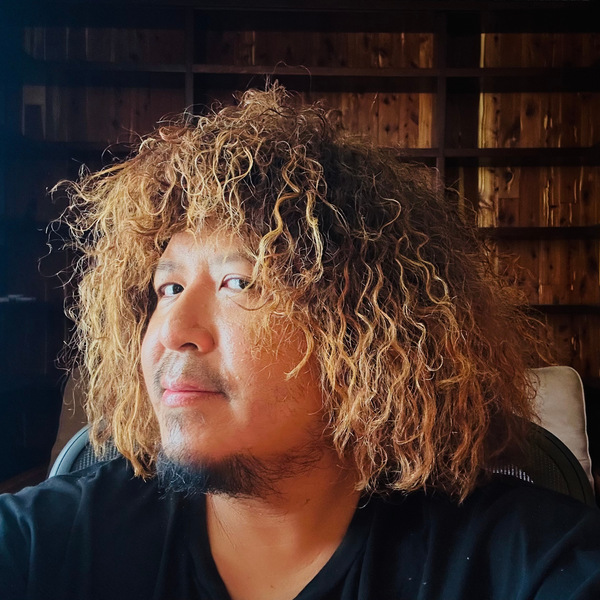
\includegraphics[width=0.09\textheight]{figures/students/tze_goh.jpg}%
            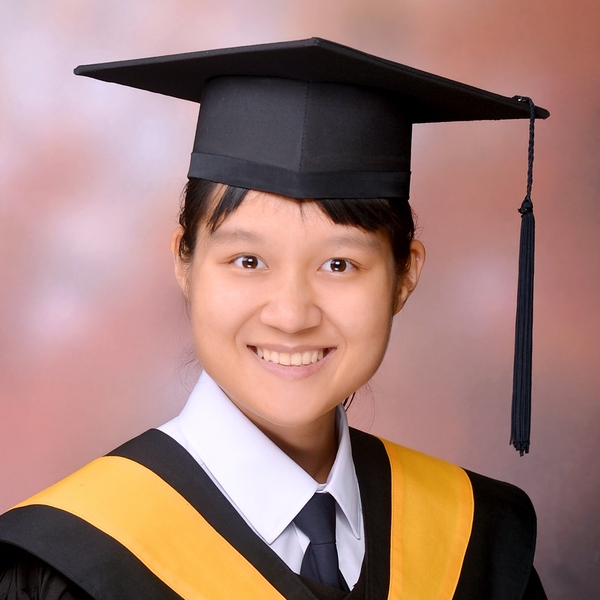
\includegraphics[width=0.09\textheight]{figures/students/wei-ning_deng.jpg}%
    };
    \begin{itemize}
        \item These musings emerged from conversations with:
            \begin{itemize}
                \item David Yallup
                \item Mike Hobson
                \item Ben Wandelt
                \item Justin Alsing
                \item Niall Jeffreys
            \end{itemize}
        \item As scientists, we should be cautious of amortised approaches
        \item \texttt{lsbi} preview: a package-driven attempt to free SBI from ML
    \end{itemize}
\end{frame}

\begin{frame}
    \frametitle{Cosmological forecasting}
    \framesubtitle{Have you ever done a Fisher forecast, and then felt Bayesian guilt?}
    \vspace{-20pt}
    \begin{columns}[t]
        \column{0.5\textwidth}
        \begin{itemize}
            \item Cosmologists are interested in forecasting what a Bayesian analysis of future data might produce.
            \item Useful for:
                \begin{itemize}
                    \item white papers/grants,
                    \item optimising existing instruments/strategies,
                    \item picking theory/observation to explore next.
                \end{itemize}
            \item To do this properly:
                \begin{enumerate}
                    \item start from current knowledge $\pi(\theta)$, derived from current data
                    \item Pick potential dataset $D\sim\mathcal{Z}(D)$ that might be collected from $P(D)\: (=\mathcal{Z})$
\item Derive posterior $\mathcal{P}(\theta|D)$
                    \item Summarise science (e.g. constraint on $\theta$, ability to perform model comparison)
                \end{enumerate}
        \end{itemize}

        \column{0.5\textwidth}
        \begin{itemize}
            \item This procedure should be marginalised over:
                \begin{enumerate}
                    \item All possible parameters $\theta$ (consistent with prior knowledge)
                    \item All possible data $D$
                \end{enumerate}
            \item i.e. marginalised over the joint $P(\theta,D)=P(D|\theta)P(\theta)$.
            \item Historically this has proven very challenging.
            \item Most analyses assume a fiducial cosmology $\theta_*$, and/or a Gaussian likelihood/posterior (c.f. Fisher forecasting).
            \item This runs the risk of biasing forecasts by baking in a given theory/data realisation.
        \end{itemize}
        
    \end{columns}

\end{frame}

\appendix
\begin{frame}
    \frametitle{Fully Bayesian Forecasting~\arxiv{2309.06942}}
    \student{thomas_gessey-jones}{Thomas Gessey-Jones}{PhD}
    \begin{columns}
        \column{0.5\textwidth}
        \begin{itemize}
            \item Simulation based inference gives us the language to marginalise over parameters $\theta$ and possible future data $D$.
            \item Evidence networks give us the ability to do this at scale for forecasting.
            \item Demonstrated in 21cm global experiments, marginalising over:
                \begin{itemize}
                    \item theoretical uncertainty
                    \item foreground uncertainty
                    \item systematic uncertainty
                \end{itemize}
            \item Able to say ``at 67mK radiometer noise'', have a 50\% chance of 5$\sigma$ Bayes factor detection.
            \item Can use to optimise instrument design
            \item Re-usable package: \texttt{prescience}
        \end{itemize}
        \column{0.5\textwidth}
        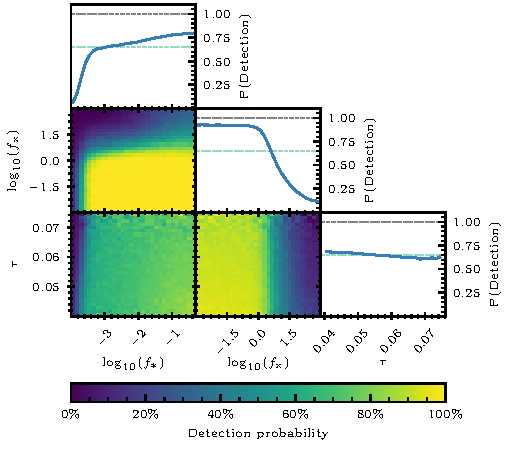
\includegraphics[width=\textwidth]{figures/fbf.pdf}
    \end{columns}
\end{frame}

\end{document}
